\documentclass[11.5pt,a4paper,russian]{article}
\usepackage[utf8]{inputenc}
\usepackage[T1,T2A]{fontenc}
\usepackage{indentfirst}
\usepackage[a4paper]{geometry}
\geometry{verbose,tmargin=1cm,lmargin=1cm,rmargin=1cm, bmargin=2cm}
\usepackage[russian]{babel}
\usepackage[warn]{mathtext}
\usepackage{caption}
\usepackage{subcaption}

\usepackage{graphicx}
\graphicspath{ {images/} }
\usepackage{tikz}
\usepackage{pgfplots}

\usepackage{amsmath}
\usepackage{floatflt}

\usepackage{multicol}
\usepackage{multirow}
\usepackage{booktabs}
% \setlength{\columnsep}{2cm}

% \usepackage{multicol}
% \setlength{\columnsep}{2cm}
\usepackage{hyperref}
\usepackage{wrapfig}

\def\AA{\mathring{\mathrm{A}}}

\begin{document}
	
\begin{titlepage}

\begin{center}

\large \textit{\small Московский физико-технический институт (государственный университет)}

\vspace{5cm}
\textit{Работа: 5.2.3}

\vspace{1cm}
\textbf{\huge Исследование спектра поглощения паров йода.}

\vspace{12cm}

\begin{flushright}
\parbox{0.45\textwidth}{
Выполнил: \\[0.5cm]
Киракосян Давид Арсенович (Б02-006) \\[0.2cm]
}
\end{flushright} 

\vfill

\today
\end{center}
\end{titlepage}

\textbf{Цель работы:} измерить спектры поглощения паров йода, выделить серии электронно-колебательных переходов, определить параметры потенциала межъядерного взаимодействия в двухатомной молекуле йода.

\textbf{В работе используются:} оптическая скамья, линза, монохроматор УМ-2 оборудованный системой цифровой регистрации изображения спектра (зеркальный цифровой фотоаппарат присоединённый к компьютеру), программное обеспечение для работы с данными raw-файлов, газоразрядные ртутная и неоновая лампы, лампа накаливания и герметичные кюветы с парами йода.

\section{Теоретические сведения}
Двухатомная молекула является сложной многочастичной устойчивой системой, состоящей из двух ядер и некоторого количества электронов. Одна из основных проблем теоретического рассмотрения молекулы – это проблема образования химической связи, обеспечивающей её устойчивость. Решение квантово-механической задачи вычисления\\
энергии основного состояния молекулы возможно лишь с привлечением приближённых методов. Благодаря этим приближениям можно рассмотреть задачу как отдельно движение электронов в электростатическом поле неподвижных ядер и движение самих ядер в некотором эффективном потенциале.

Сначала решается задача для движения электронов в поле неподвижных ядер. Для каждой конфигурации положений ядер $\{ R_i \}$ решение электронной задачи определяет значение энергии электронной подсистемы – $E_n^{el}$.

На следующем шаге решается задача для движения ядер, при этом к энергии электростатического отталкивания ядер добавляется энергия электронной подсистемы: $U_n^{e f f}\left(\left\{\vec{R}_i\right\}\right)=U_\text{я}\left(\left\{\vec{R}_i\right\}\right)+E_n^{e l}$. Эта эффективная энергия взаимодействия ядер в молекуле называется \textit{электронным термом} молекулы, а саму зависимость $U_n^{e f f}\left(\left\{\vec{R}_i\right\}\right)$ - потенциальной кривой электронного терма с номером $n$. Различным стационарным энергетическим уровням электронной подсистемы будут соответствовать различные электронные термы молекулы.

\subsection{Вращательные уровни и вращательный спектр.}
Рассмотрим вращательное движение молекулы. В первом приближении можно считать, что молекула представляет собой жесткий ротатор, то есть расстояние между атомами молекулы не зависит от энергии ее вращения, которая определяется следующим выражением:

$$
E = \dfrac{1}{2}I\omega^2 = \dfrac{p^2}{2I},
$$

где $\omega$ — круговая частота вращения, $I$ — момент инерции молекулы и $p = I\omega$ — момент количества движения. Согласно квантовой механике, квадрат момента количества движения может принимать лишь дискретные значения:

\[p^2 = \dfrac{h^2}{4\pi^2} j(j+1),~j=0,1,2,\dots\text{ -- вращательное квантовое число.}.\]

Получаем для энергии вращения выражение:

\[E_j = \dfrac{\hbar^2}{2I}j(j+1),\]

или если выражать энергию в обратных сантиметрах, то

\begin{equation}
E_j = \dfrac{E_j}{hc} = \dfrac{h}{8\pi^2Ic}j(j+1) \stackrel{\mathrm{def}}{=} B j (j+1).
\label{1}
\end{equation}

Чисто вращательным спектром обладают линейные молекулы с ненулевыми постоянным дипольным моментом. Разрешенный переход для вращательных уровней удовлетворяет условию

\[\Delta j = j' - j'' = \pm 1.\]

При этом энергия переходов определяется выражением \eqref{1} и равна

\[\Delta E = 2Bj'.\]

Отсюда видно, что вращательный спектр должен состоять из ряда равноотстоящих линий. Однако приближение жесткого ротатора оказывается неточным для большинства реальных молекул. Для лучшего приближения наблюдаемой картины необходимо ввести влияние центробежного растяжение путем введения величины $D$:

\[E_j = Bj(j+1) - Dj^2(j+1)^2.\]

Величина $D$ почти на пять порядков меньше величины $B$, поэтому такая поправка оказывается значимой только при больших значениях вращательного квантового числа $j \geq 10$.

\section{Колебательные уровни и колебательный спектр.}
Для описания колебательного движения атомов в молекуле в основном используются две модели: модель гармонического и ангармонического осциллятора.

Модель гармонического осциллятора является наиболее простой моделью и позволяет корректно описывать положение нижних колебательных уровней молекулы. Энергия уровней в такой модели определяется формулой

\[E_v = \omega_e\left(v + \dfrac{1}{2} \right), ~\left[ \text{см}^{-1} \right]\]

где $v = 0, 1, 2, \dots$ -- колебательное квантовое число, $\omega_e$ -- собственная частота осциллятора, выраженная в $\text{см}^{-1}$. Для колебательных переходов гармонического осциллятора выполняется простое правило отбора:

\[\Delta v = \pm 1.\]

Применяя его, находим, что частота излучения, соответствующего колебательным переходам, не зависит от номера уровня и составляет

\[E_{v+1 \rightarrow v} = \omega_e.\]

Реальные молекулы не следуют точно законам гармонического осциллятора, и чем больше колебательная энергия молекулы, тем сильнее наблюдаемое отличие. Для более точного описания колебательного движения молекулы используется модель ангармонического осциллятора. В качестве эффективного потенциала $U_n^{e f f}$ выбирают потенциал \textit{Морзе}.

$$
U^{e f f}(\rho)=A\left(e^{-2 \alpha\left(\rho-\rho_0\right)}-2 e^{-\alpha\left(\rho-\rho_0\right)}\right)+D
$$

Характерный вид этой зависимости и соответствующие обозначения показаны на рисунке \ref{fig:morze}.

\begin{figure}[h!]
  \centering
  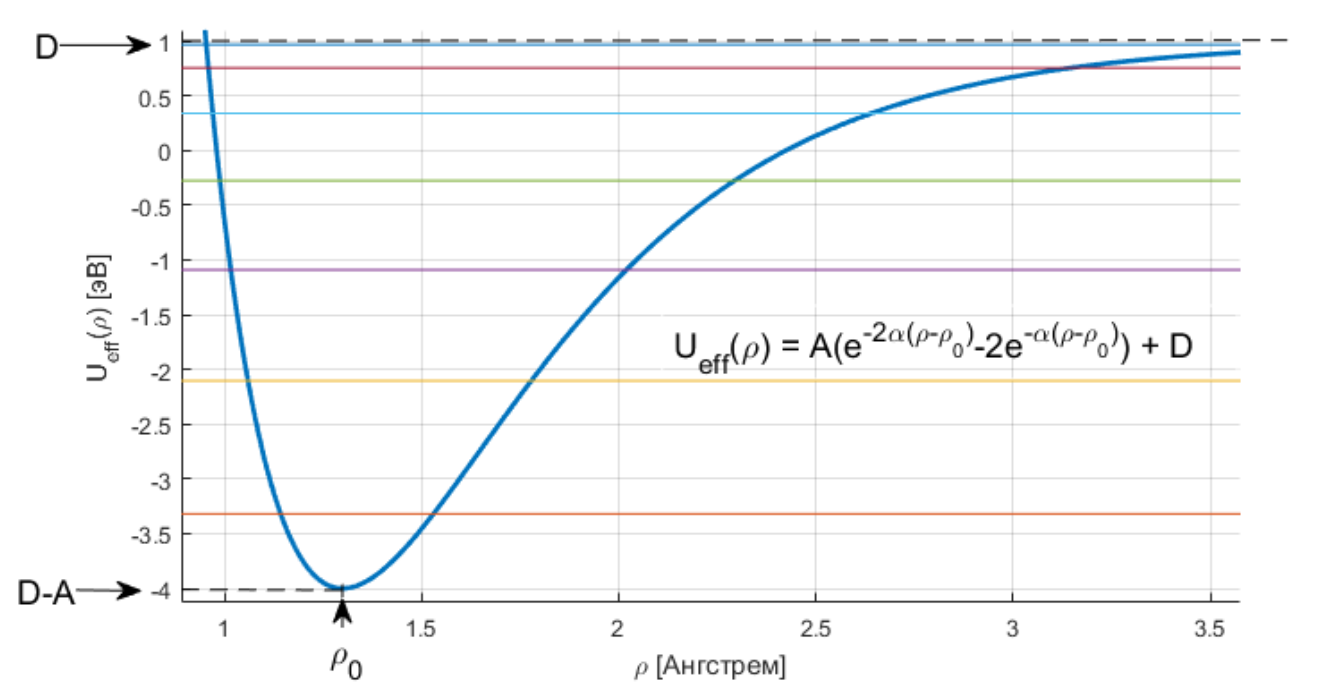
\includegraphics[width=\textwidth]{156e090e-cae2-483e-83c2-33e40d83edd8}  \caption{Потенциал Морзе}
  \label{fig:morze}
\end{figure}

На графике также показаны энергетические уровни стационарных состояний для одномерного движения в таком потенциале, соответствующие колебательным термам. Отличительной особенностью энергетического спектра этого потенциала является конечное число дискретных уровней и уменьшение расстояния между соседними энергетическими уровнями с повышением номера уровня. Выражение для энергетического спектра движения в потенциале Морзе имеет вид:

$$
E_n=D-A+\hbar \alpha \sqrt{\frac{2 A}{\mu}}\left(n+\frac{1}{2}\right)-\frac{\hbar^2 \alpha^2}{2 \mu}\left(n+\frac{1}{2}\right)^2
$$

Обозначив частоту колебательного кванта $\omega_{\text {кол }}=\alpha \sqrt{\frac{2 A}{\mu}}$ можно переписать в виде:

\begin{equation}\label{eq:E}
E_n=D-A+\hbar \omega_{\text {кол }}\left(n+\frac{1}{2}\right)-\frac{1}{4 A}\left(\hbar \omega_{\text {кол }}\left(n+\frac{1}{2}\right)\right)^2
\end{equation}

Для анализа такого спектра полезно записать выражения для разностей между соседними уровнями $\Delta E_n=E_{n+1}-E_n$ :

\begin{equation}\label{eq:deltaE}
\Delta E_n=\hbar \omega_{\text {кол }}-\frac{\hbar^2 \alpha^2}{\mu}(n+1)=\hbar \omega_{\text {кол }}\left(1-\frac{\hbar \omega_{\text {кол }}}{2 A}(n+1)\right)
\end{equation}

и выражение для вторых разностей $\Delta^2 E_n=\Delta E_{n+1}-\Delta E_n$ :

\begin{equation}\label{eq:delta2E}
\Delta^2 E_n=-\frac{\hbar^2 \alpha^2}{\mu}=-\frac{\left(\hbar \omega_{\text {кол }}\right)^2}{2 A}
\end{equation}

Для случая потенциала Морзе, значение вторых разностей одинаково для всего спектра, не зависит от номера $n$. Используя выше полученные выражения и экспериментально измеренный колебательный спектр можно вычислить микроскопические параметры $\alpha$ и $A$ описывающие взаимодействие между ядрами в двуатомной молекуле.

\subsection{Принцип Франка-Кондона}
Как отмечено выше, различные состояния электронной подсистемы соответствуют различным электронным термам молекулы. Переходы между электронными термами могут сопровождаться электромагнитным излучением на частотах вблизи видимого диапазона. Точное значение частоты излучения определяется не только электронными термами начального и конечного состояний молекулы, но ещё и соответствующими колебательными и вращательными термами.

Вероятность излучательного перехода зависит от матричного элемента дипольного момента $\left|\mathbf{d}_{12}\right|^2$. Для сферически симметричных систем условие $\left|\mathbf{d}_{12}\right|^2 \neq 0$ приводит к так называемым правилам отбора, которые связаны с законом сохранения момента импульса и чётности при переходе между квантовыми состояниями. Но для двухатомных молекул ${ }^7$ возникает специфическое правило, определяющее вероятность излучательного перехода - так называемый принцип Франка-Кондона.

Для пояснения этого принципа на рисунке \ref{fig:frank_condon} показаны потенциальные кривые двух различных электронных термов, а также колебательные термы каждого электронного состояния. Вращательные термы не показаны. Помимо энергетических уровней стрелочками обозначена серия поглощающих переходов $\left(n-n^{\prime}\right)$ и серия испускающих переходов $\left(n^{\prime}-n\right)$.\\
В наиболее простой формулировке принцип Франка-Кондона гласит, что интеграл перекрытия волновых функций состояний $(n)$ и $(n')$ определяет вероятность излучательного перехода между этими состояниями, и чем выше значения интеграла $\langle n | n' \rangle$, т.е. перекрытие волновых функций, тем выше вероятность такого перехода.

\begin{wrapfigure}{r}{0.4\textwidth}
  \centering
  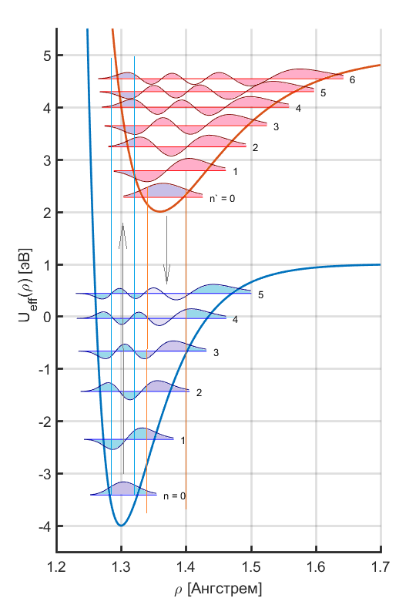
\includegraphics[width=0.4\textwidth, height=0.4\textwidth]{467e288a-4953-41fa-b857-148b8fde2aa7}
  \caption{Электронно-колебательные термы и переходы}
  \label{fig:frank_condon}
  \vspace{-1cm}
\end{wrapfigure}

\section{ Экспериментальная установка}
\subsection{Схема экспериментальной установки}
Установка для измерения спектров включает в себя оптическую скамью, источники излучения (газоразрядную ртутную лампу и лампу накаливания), кювету с парами йода, фокусирующую линзу и монохроматор с установленным на нём цифровым зеркальным фотоаппаратом. Источники излучения, кювета и линза устанавливаются на оптической скамье, которая жёстко соединена с корпусом монохроматора. Общая схема установки показана на рисунке \ref{fig:ustanovka}.

Излучение подаётся через коллимационную линзу на входную щель монохроматора, и пройдя через линзы и призму, фокусируется на плоскости светочувствительной матрицы фотоаппарата.

\subsection{Устройство цифрового оптического спектрометра}
Для измерения оптических спектров в работе используется используется призменный монохроматор УМ-2 оборудованный цифровым фотоаппаратом Canon EOS 650D или Nikon D5300. Также возможен вариант с использованием монохроматора ИСП51. Цифровой фотоаппарат установлен вместо выходного окуляра монохроматора, так что изображение спектра формируется прямо на фоточувствительную матрицу. Использование цифрового фотоаппарата в качестве регистрирующего устройства позволяет повысить точность и чувствительность измерений, а также даёт возможность собрать большее количество данных и пронаблюдать более тонкие эффекты. При этом остаётся, по прежнему, возможность наблюдать спектр изучаемого излучения непосредственно глазом. Для этого достаточно опустить зеркало фотоаппарата в исходное положение.

\begin{figure}[h!]
  \centering
  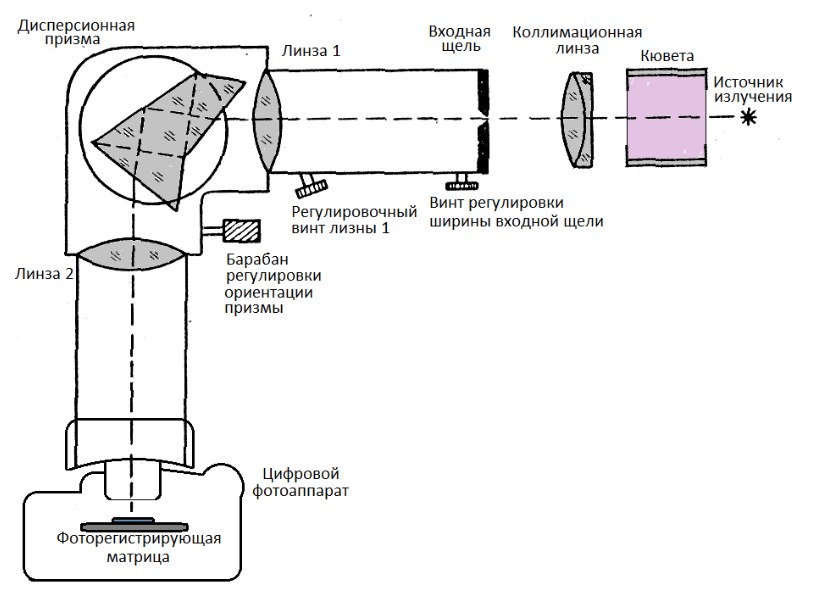
\includegraphics[width=0.7\textwidth]{147ff95c-a921-4ffa-b390-beb2908f24cf}  \caption{Схема установки регистрации оптических спектров}
  \label{fig:ustanovka}
\end{figure}

Фотоаппарат подключён к персональному компьютеру с помощью USB кабеля. C помощью поставляемой производителем фотоаппарата программы EOS Utility (Camera Control Pro - для Nikon D5300) можно осуществлять управление фотоаппаратом с компьютера и получать изображение формируемое на матрице фотоаппарата на экране монитора в режиме реального времени.

Получаемые фотографии сохраняются сразу на жёсткий диск компьютера. Регистрируемые данные записываются в файлы в raw-формате. В дальнейшем данные из этих файлов обрабатываются с помощью программы VisSpectra, которая позволяет выделить из этих raw-фотографий спектральные зависимости интенсивности излучения, а также провести спектральную калибровку.

\section{Ход работы}

\begin{figure}[ht!]
\centering
    \begin{subfigure}[b]{0.3\textwidth}
  \centering
  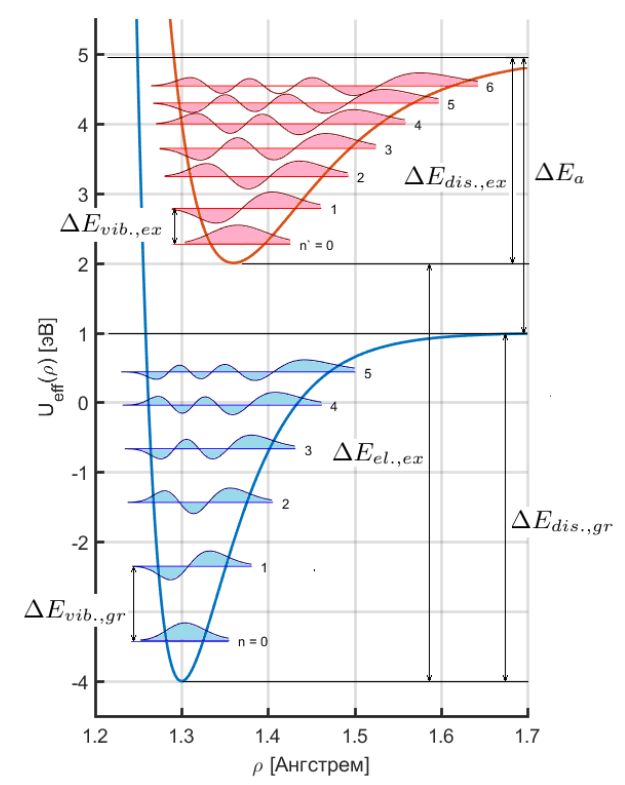
\includegraphics[width=\textwidth]{31d5f3f2-62f2-4406-9102-ef96d1b02bcb}  \caption{Уровни энергии переходов}
  \label{fig:analyze_problem}
\end{subfigure}
\begin{subfigure}[b]{0.4\textwidth}
  \centering
  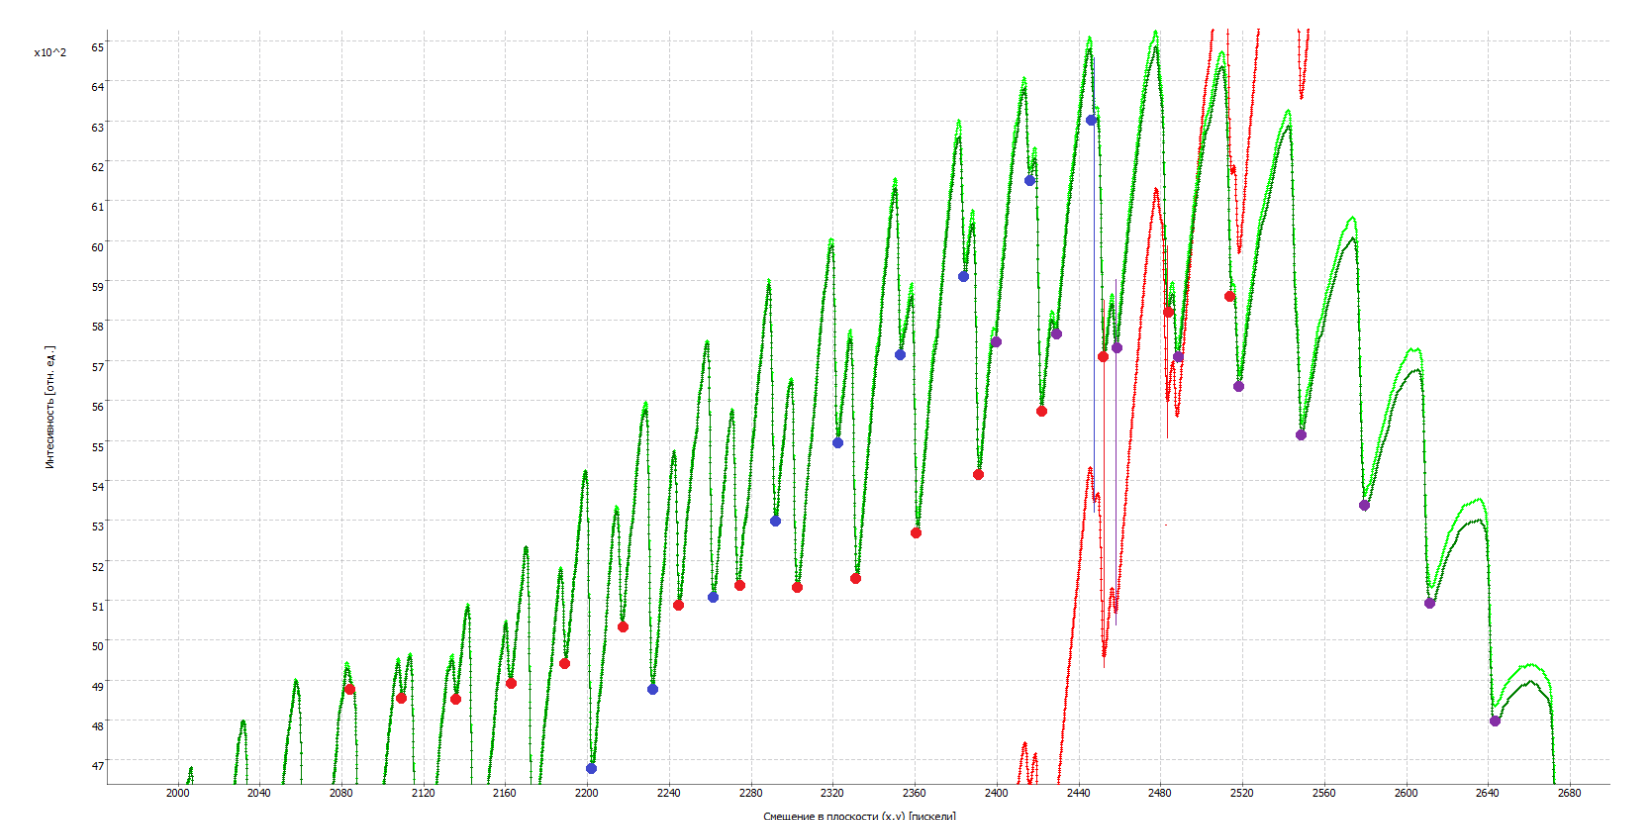
\includegraphics[width=\textwidth]{215eb016-6116-47f0-b2c0-8b7fd67629ac}  \caption{Фрагмент спектра поглощения паров йода с выделенными тремя различными сериями линий поглощения.}
  \label{fig:series}
\end{subfigure}
\end{figure}

Получим серии переходов из электронно-колебательных спектров. Вид такого спектра и серий приведены на рисунке \ref{fig:series}. Калибровка спектров была проведена с помощью спектра излучения ртутной лампы. Результаты измерений приведены в таблице \ref{table:data}

\begin{table}[b]
\centering
\caption{Результаты измерений серий}\
\label{table:data}
\begin{tabular}{c|c|c|c|c|c||c|c|c|c|c|c}
\toprule
№ Серии & n & $l$, $\AA$ & $\sigma_l$, $\AA$ & $E$, эВ & $\sigma_E, 10^{-4}$  эВ & № Серии & n & $l$, $\AA$ & $\sigma_l$, $\AA$ & $E$, эВ & $\sigma_E, 10^{-4}$  эВ \\
\midrule
1 & 0 & 5742.3 & 0.5 & 2.159 & 1.99 & 2 & 4 & 5686.7 & 0.3 & 2.180 & 1.07 \\
1 & 1 & 5710.2 & 0.4 & 2.171 & 1.34 & 2 & 5 & 5657.1 & 0.6 & 2.192 & 2.16 \\
1 & 2 & 5679.0 & 0.4 & 2.183 & 1.36 & 2 & 6 & 5629.0 & 0.6 & 2.203 & 2.18 \\
1 & 3 & 5647.9 & 0.2 & 2.195 & 0.69 & 2 & 7 & 5600.5 & 0.6 & 2.214 & 2.20 \\
1 & 4 & 5618.2 & 0.4 & 2.207 & 1.39 & 2 & 8 & 5574.3 & 0.6 & 2.224 & 2.22 \\
1 & 5 & 5589.5 & 0.2 & 2.218 & 0.70 & 2 & 9 & 5547.8 & 0.6 & 2.235 & 2.25 \\
1 & 6 & 5561.5 & 0.3 & 2.229 & 1.06 & 2 & 10 & 5523.0 & 0.6 & 2.245 & 2.27 \\
1 & 7 & 5534.7 & 0.3 & 2.240 & 1.07 & 2 & 11 & 5498.5 & 0.8 & 2.255 & 3.43 \\
1 & 8 & 5508.5 & 0.3 & 2.251 & 1.08 & 2 & 12 & 5474.8 & 0.6 & 2.265 & 2.31 \\
1 & 9 & 5483.4 & 0.4 & 2.261 & 1.46 & 2 & 13 & 5451.9 & 0.6 & 2.274 & 2.33 \\
1 & 10 & 5459.3 & 0.3 & 2.271 & 1.10 & 3 & 0 & 6242.0 & 1.5 & 1.986 & 4.79 \\
1 & 11 & 5435.6 & 0.4 & 2.281 & 1.48 & 3 & 1 & 6198.7 & 0.4 & 2.000 & 1.21 \\
1 & 12 & 5412.7 & 0.3 & 2.291 & 1.12 & 3 & 2 & 6155.9 & 0.8 & 2.014 & 2.46 \\
1 & 13 & 5390.8 & 0.4 & 2.300 & 1.51 & 3 & 3 & 6114.5 & 0.8 & 2.028 & 2.49 \\
1 & 14 & 5369.2 & 0.4 & 2.309 & 1.52 & 3 & 4 & 6074.7 & 0.8 & 2.041 & 2.53 \\
1 & 15 & 5348.2 & 0.3 & 2.318 & 1.15 & 3 & 5 & 6035.6 & 0.8 & 2.054 & 2.56 \\
1 & 16 & 5329.0 & 0.3 & 2.327 & 1.16 & 3 & 6 & 5996.8 & 0.8 & 2.067 & 2.59 \\
1 & 17 & 5309.9 & 0.3 & 2.335 & 1.17 & 3 & 7 & 5959.2 & 0.8 & 2.081 & 2.63 \\
1 & 18 & 5291.2 & 0.3 & 2.343 & 1.17 & 3 & 8 & 5922.0 & 0.8 & 2.094 & 2.66 \\
1 & 19 & 5274.1 & 0.3 & 2.351 & 1.18 & 3 & 9 & 5886.7 & 0.8 & 2.106 & 2.69 \\
1 & 20 & 5257.3 & 0.4 & 2.358 & 1.59 & 3 & 10 & 5851.7 & 0.8 & 2.119 & 2.72 \\
1 & 21 & 5240.8 & 0.3 & 2.366 & 1.20 & 3 & 11 & 5818.6 & 1.1 & 2.131 & 4.13 \\
1 & 22 & 5225.6 & 0.3 & 2.373 & 1.20 & 3 & 12 & 5785.9 & 0.8 & 2.143 & 2.78 \\
1 & 23 & 5210.9 & 0.3 & 2.379 & 1.21 & 3 & 13 & 5754.3 & 0.8 & 2.155 & 2.82 \\
1 & 24 & 5196.1 & 0.3 & 2.386 & 1.22 & 4 & 0 & 6421.3 & 0.8 & 1.931 & 2.26 \\
1 & 25 & 5183.4 & 0.3 & 2.392 & 1.22 & 4 & 1 & 6374.3 & 0.8 & 1.945 & 2.29 \\
1 & 26 & 5169.7 & 0.1 & 2.398 & 0.41 & 4 & 2 & 6327.3 & 0.8 & 1.960 & 2.33 \\
1 & 27 & 5157.3 & 0.2 & 2.404 & 0.82 & 4 & 3 & 6281.5 & 0.4 & 1.974 & 1.18 \\
1 & 28 & 5145.4 & 0.2 & 2.410 & 0.82 & 4 & 4 & 6237.8 & 0.8 & 1.988 & 2.40 \\
1 & 29 & 5134.2 & 0.2 & 2.415 & 0.83 & 4 & 5 & 6195.0 & 0.8 & 2.001 & 2.43 \\
2 & 0 & 5813.8 & 0.3 & 2.133 & 1.02 & 5 & 0 & 6557.8 & 0.8 & 1.891 & 2.17 \\
2 & 1 & 5781.2 & 0.3 & 2.145 & 1.03 & 5 & 1 & 6509.3 & 0.4 & 1.905 & 1.10 \\
2 & 2 & 5748.5 & 0.6 & 2.157 & 2.09 & 5 & 2 & 6460.4 & 0.4 & 1.919 & 1.12 \\
2 & 3 & 5717.3 & 0.3 & 2.169 & 1.06 & 5 & 3 & 6412.8 & 0.8 & 1.933 & 2.27 \\
2 & 4 & 5686.7 & 0.3 & 2.180 & 1.07 & 5 & 4 & 6365.7 & 0.8 & 1.948 & 2.30 \\
- & - & - & - & - & - & 5 & 5 & 6320.2 & 0.8 & 1.962 & 2.33 \\
\bottomrule
\end{tabular}
\end{table}

Используя данные полученные из спектральных измерений можно вычислить на их основе следующие параметры молекулы йода: величину колебательного кванта для возбуждённого электронного терма $\Delta E_{v i b ., e x}$ и, аналогично, для основного электронного терма $\Delta E_{v i b ., g r}$, оценить величину энергии между дном основного электронного терма и дном возбуждённого электронного терма $\Delta E_{e l ., e x}$, оценить энергию, необходимую для диссоциации молекулы находящейся на возбуждённом электронном терме $\Delta E_{\text {dis.,ex }}$. Определить энергию диссоциации молекулы на основном электронном терме $\Delta E_{\text {dis.,gr }}$ и энергию возбуждения $\Delta E_a$ отдельного атома йода. Для большей ясности, на рисунке \ref{fig:analyze_problem} эти значения энергии указаны как интервалы относительно линий энергетического спектра колебательных состояний двухатомной молекулы. Для определения этих параметров необходимо обработать данные полученных серий спектральных минимумов.

\begin{enumerate}
  \item Для каждой серии вычислить значения первых разностей уровней энергии $\Delta E_{n_m}=E_m(n+1)-E_m(n)$, соответствующих формуле \eqref{eq:deltaE} Номера серий $m$ назначать так, чтобы большему номеру серии $m$ cоответствовала меньшая минимальная энергия линии поглощения в серии. $\left(E_1(0)>E_2(0)>E_3(0)>\ldots\right)$
  \item Построим графики зависимостей значений первых разностей энергии уровней от номера этого значения в серии.
\end{enumerate}

\begin{figure}[h!]
  \centering
  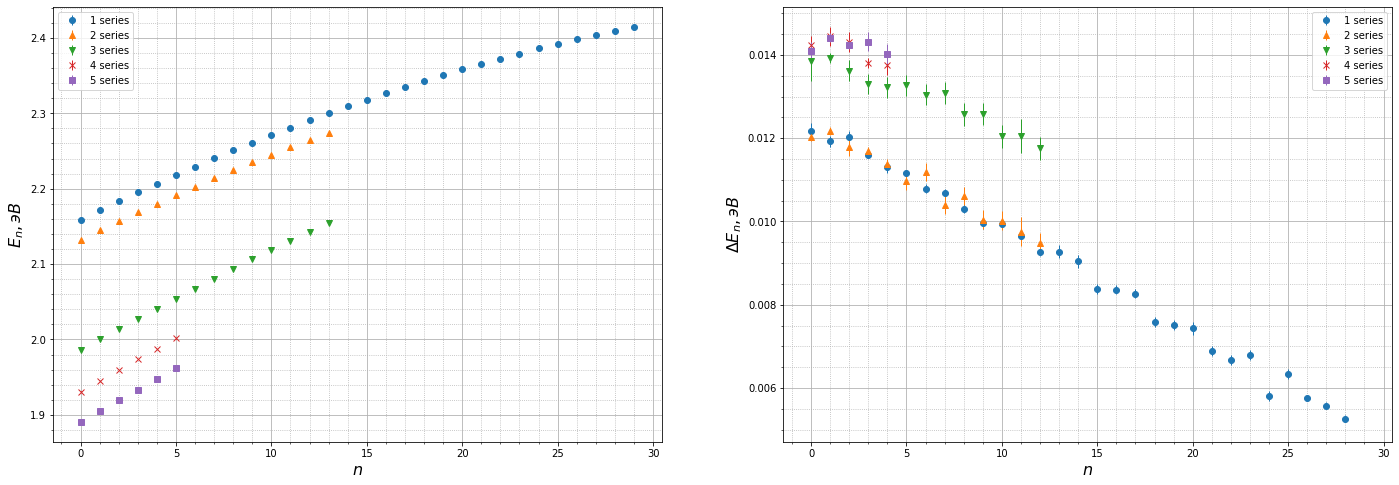
\includegraphics[width=\textwidth]{4246b306-1dae-4c38-90dc-b70b657b2cbb}  \caption{График серии переходов (слева) и первых разностей (справа)}
\end{figure}

\begin{enumerate}
  \setcounter{enumi}{2}
  \item Подберем значения индексов смещения линий поглощения для каждой серии, такие, чтобы все зависимости укладывались в одну общую зависимость, то есть лежали на одной прямой. После определения индексов смещения построим график и зависимостей энергий для каждой серии с учётом индексов смещения
\end{enumerate}

\begin{figure}[h!]
  \centering
  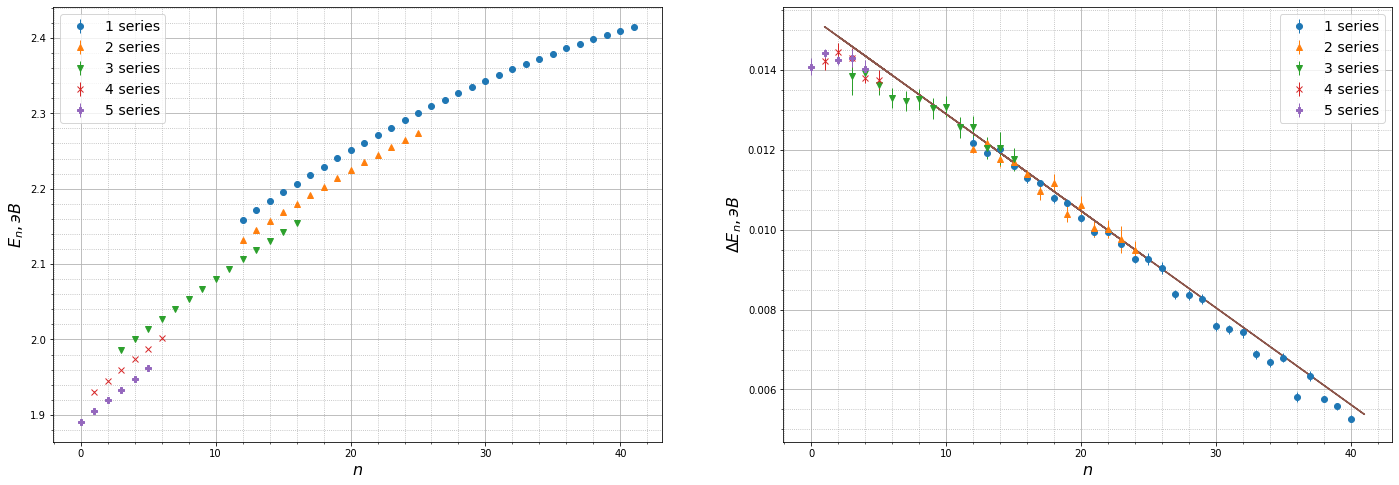
\includegraphics[width=\textwidth]{aeedd2af-8426-4789-b56d-b3a72c19f729}  \caption{График серий и первых разностей возбужденного уровня после смещений индексов $n$}
  \label{fig:1_diff}
\end{figure}

\newpage

\begin{enumerate}
  \setcounter{enumi}{3}
  \item Убедимся что в области пересечения графиков для различных серий, разница между энергиями остаётся примерно одинаковой. Вычислить средние значения такой разницы для всех пар соседних серий. Построим зависимость этой величин от номера серии -- это будет график первых разностей энергий для основного электронного терма. Из этого графика определим квант колебательного движения основного электронного терма – $\Delta E_{v i b ., g r}$
\end{enumerate}

\begin{figure}[h!]
  \centering
  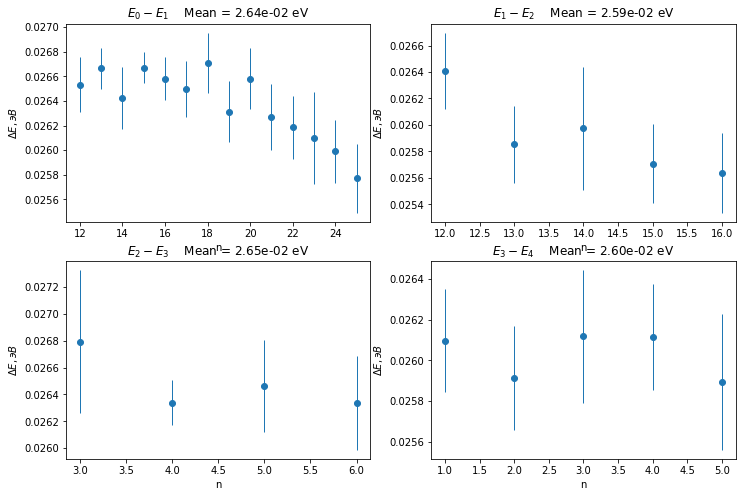
\includegraphics[width=\textwidth]{df661de4-e395-41d0-898a-280d23e4e92b}
\end{figure}

$\Delta E_{v i b ., g r}$ является средняя энергия всех этих разностей.

$$
\Delta E_{v i b ., g r} = (26.8 \pm 0.5) 10^{-3} \text{эВ}
$$

Для каждой пар серий посчитаем среднее и построим графики этой зависимости от номера серии.

\begin{figure}[h!]
  \centering
  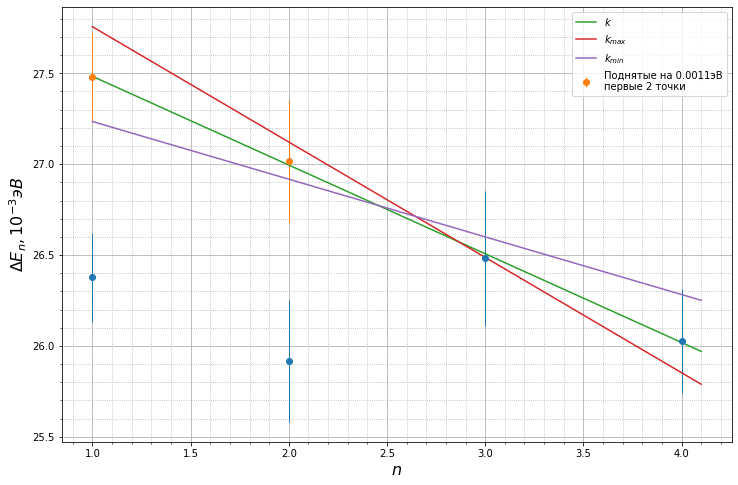
\includegraphics[width=0.8\textwidth]{17dfeaf6-744c-448d-8d25-7ecdcdc88a9c}
  \caption{График средней разности энергий для каждых соседних пар}
\end{figure}

Заметим что первые две точки (соответствующие n=1, 2) находятся на $0.0011$эВ ниже линии проходящее через последние две точки. Скорее всего при определении смещений первых двух серий возникла систематическая ошибка. Следовательно поднимем эти точки на 0.0011 эВ и построим прямую через эти две точки. Для определения погрешности наклона определим $k_{min}, k_{max}$ проходящее через областей погрешности точек.\\
В итоге получаем

$$
\Delta^2 E_{gr} = - (4.8 \pm 1.4) \cdot 10^{-4} \text{эВ}
$$

\begin{enumerate}
  \setcounter{enumi}{4}
  \item Определим из графика значений первых разностей для возбужденного электронного терма (Рис. \ref{fig:analyze_problem} справа) соответствующий колебательный квант $\Delta E_{v i b ., e x}$ и значение вторых разниц для возбужденного терма $\Delta^2 E_{ex}$.\\
\begin{align}
\Delta E_{v i b ., e x} &= (15.33 \pm 0.06) \cdot 10^{-3} \text{эВ} \\
\Delta^2 E_{ex} &= (2.43 \pm 0.02) \cdot 10^{-4} \text{эВ}
\end{align}

  \item Теперь найдем величину энергии между дном основного электронного терма и дном возбуждённого электронного терма $\Delta E_{el, ex}$. Для этого нужно продолжить параболой 1 серию (серия переходов из 0 невозбужденного терма в возбужденные термы).\\
В итоге получим

\end{enumerate}

\begin{figure}[h!]
  \centering
  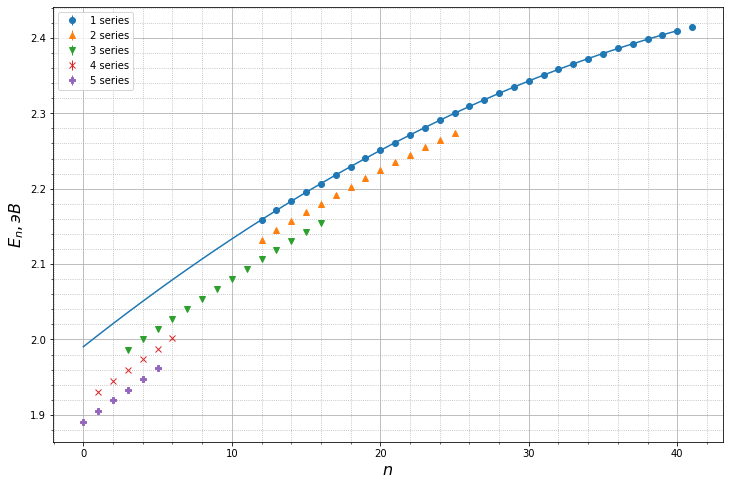
\includegraphics[width=0.8\textwidth]{6ff35e60-3113-41e5-823f-6d8197fa322a}  \caption{Приближение 1 серии параболой}
  \label{fig:fit_parabola}
\end{figure}

\begin{gather*}
E^{(1)}_n = W_2 + W_1 \left(n+\frac12 \right) + W_0 \left(n+\frac12 \right)^2 \\
W_0 = -1.27 \cdot 10^{-4} \text{эВ} \quad W_1 = 1.57 \cdot 10^{-2} \text{эВ} \quad W_2 = 1.98 \text{эВ} \\
\varepsilon_W < 1 \%
\end{gather*}

$W_2$ является разницей между энергиями $n=0$ невозбужденного терма и дном основного электронного терма (Рис. \ref{fig:analyze_problem}). Следовательно

$$
\Delta E_{el, ex} = W_2 + \frac{\hbar \omega_e}{2} = W_2 + \frac{\Delta E_{v i b ., g r}}2 = (1.99 \pm 0.01) \text{эВ}
$$

\begin{enumerate}
  \setcounter{enumi}{6}
  \item По формуле (\eqref{eq:delta2E}) вычислить параметры $\alpha_{gr}$ и $\alpha_{ex}$ потенциала Морзе, аппроксимирующего потенциальную кривую основного и возбуждённого электронного термов. Для $\mathrm{I}_2$ приведенная масса $\mu = 63.5 \, \text{а.м.}$.\\
\begin{gather*}
  \alpha_{gr} = \frac{\sqrt{-\mu \Delta^2 E_{gr} }} {\hbar} = (2.7 \pm 0.4) \cdot 10^{10} \text{м}^{-1} \\ 
  \alpha_{ex} = \frac{\sqrt{-\mu \Delta^2 E_{ex} }} {\hbar} = (1.92 \pm 0.02) \cdot 10^{10} \text{м}^{-1}
\end{gather*}

  \item Оценим полное число $N_{gr}$ и $N_{ex}$ колебательных уровней основного и возбуждённого электронных термов. Сначала выведем необходимую формулу из вида энергетического спектра потенциала Морзе (\eqref{eq:E}).
\begin{gather*}
E_N = D-A + \hbar \omega_e \left(N+\frac12 \right) - \frac{(\hbar \omega_e)^2}{4A}\left(N+\frac12 \right)^2 \approx D \Rightarrow \\
N + \frac12 = \dfrac{
\frac{\hbar \omega_e}{2}}{\frac{(\hbar \omega_e)^2}{4A}} = 2 \frac{A}{\hbar \omega_e} = \frac{\Delta E}{\Delta^2 E} \\
\\
N_{gr} = (62 \pm 18) \\
N_{ex} = (54 \pm 1) \\
\end{gather*}

9. Определим энергию диссоциации основного $\Delta E_{d i s ., gr}$ и возбуждённого $\Delta E_{dis.,ex }$ электронных термов, а также энергию возбуждения атома йода $\Delta E_a$\\
\begin{gather*}
\Delta E_{dis.} = D - (D-A) = A = \frac12 \frac{(\Delta E)^2}{\Delta^2 E} \\
\Delta E_{d i s ., gr} = (0.73 \pm 0.2) \text{эВ} \\
\Delta E_{d i s ., ex} = (0.486 \pm 0.001) \text{эВ} \\
\end{gather*}

\end{enumerate}

$$
\Delta E_a = \Delta E_{el ., ex} + \Delta E_{d i s ., ex} - \Delta E_{d i s ., gr} = (1.7 \pm 0.5) \text{эВ}
$$

\section{Вывод}
В ходе работы был изучен спектр поглощения паров йода, были получены параметры потенциала Морзе для $\mathrm{I}_2$, а именно:

\begin{enumerate}
  \item $\Delta E_{v i b ., g r} = (26.8 \pm 0.5) 10^{-3}$ эВ, $\Delta E^{\text{табл.}}_{v i b ., g r} = 26.5 \cdot 10^{-3}$ эВ
  \item $\Delta E_{vib, ex} = (15.33 \pm 0.06)$ эВ,  $\Delta E^{\text{табл.}}_{v i b ., ex} = 14.9 \cdot 10^{-3}$ эВ
  \item $\Delta E_{el, ex} = (1.99 \pm 0.01)$ эВ,
  \item $\Delta E_{d i s ., gr} = (0.73 \pm 0.2)$ эВ,
  \item $\Delta E_{d i s ., ex} = (0.486 \pm 0.001)$ эВ
  \item $\Delta E_a =  (1.7 \pm 0.5)$ эВ,  $\Delta E^{\text{табл.}}_{a} = 0.94$ эВ
\end{enumerate}

Несоответствие энергии возбуждения атома йода с табличным значением вызвано скорее всего из-за большой неточности определения второй разницы основного терма.


\end{document}